\section{Design}\label{sec-design}
%\section{Design}\label{sec-design}



%As described in Sec.~\ref{sec-CAT}, a confidential attestation process encompasses a standard Intel attestation to attest the bootstrap enclave and establish a secure communication channel. If they are convinced that the bootstrap enclave can enforce the desired security policies, the data or code providers can send the data and code (in encrypted form) to the bootstrap enclave. 

In this section we present our design, which elevates the SGX platform with the support for the \textsc{Deflection} model. This is done using an in-enclave software layer -- the bootstrap enclave running the code consumer and an out-enclave auxiliary -- the code generator. Following we first describe the general idea behind our design and then elaborate the policies it supports, its individual components and potential extension.     


%under the privacy preserving data processing scenario. In this setting, the service user (i.e., the data owner) communicates with the remote data processing service with encrypted messages for uploading her data and receiving the results.
%sends and receives  from remote parties. The service provider is with the infrastructure's side so that the code can be conveyed directly into the bootstrap enclave. 
%To minimize the size of the bootstrap enclave, the design borrows the idea of PCC and consists of an untrusted code producer outside the enclave, and a trusted code consumer inside.
%Sec.~\ref{subsec-threat} presents the threat model. 
%Sec.~\ref{subsec-policies} presents the categorized security policies enforced by the bootstrap enclave. Sec.~\ref{subsec-producer} and Sec.~\ref{subsec:verify} presents how the policies can be enforced and verified with the cooperative design of the code producer and code consumer. We will discuss how to extend the design to other scenarios with carefully crafted security policies in Sec.~\ref{subsec:morescenario}. 


%In this section we present our design for realizing the CAT model under the privacy preserving data processing scenario. In this setting, the service user (i.e., the data owner) communicates with the remote data processing service with encrypted messages for uploading her data and receiving the results.
%sends and receives  from remote parties. The service provider is with the infrastructure's side so that the code can be conveyed directly into the bootstrap enclave. To minimize the size of the bootstrap enclave, the design borrows the idea of PCC and consists of an untrusted code producer outside the enclave, and a trusted code consumer inside.Sec.~\ref{subsec-threat} presents the threat model. Sec.~\ref{subsec-policies} presents the categorized security policies enforced by the bootstrap enclave. Sec.~\ref{subsec-producer} and Sec.~\ref{subsec:verify} presents how the policies can be enforced and verified with the cooperative design of the code producer and code consumer. We will discuss how to extend the design to other scenarios with carefully crafted security policies in Sec.~\ref{subsec:morescenario}. 


%with little or no modification since the code generator and the policy-compliance verifier can work perfectly independently and have no impact on one another.




\subsection{Overview}
\label{subsec-overview}

\noindent\textbf{Idea}. Behind the design of \textsc{Deflection} is the idea of PCC, which enables efficient in-enclave verification of \revise{mobile code with proof}. A direct application of the existing PCC techniques, however, fails to serve our purpose, as mentioned earlier, due to the huge TCB introduced, the large proof size and the exponential time with regards to the code size for proof generation. To address these issues, we design a lightweight 
approach with an untrusted code producer and a trusted code consumer running inside the bootstrap enclave. The producer compiles the source code of the target program with necessary libraries (for service providing), generates a list of its indirect jump targets, and instruments it with security annotations (in assembly with structured inline guards) for runtime mediation of its control flow and key operations, in compliance with security policies. The list and security annotations constitute a ``proof'', which is verified by the consumer (according to certain formats) after loading the code into the enclave and before the target binary is activated. 
%\weijie{proof/annotation: assembly with certain format/inline guards, inspired by the typed x86 assembly}

%The overview design is derived from the original PCC idea while we have simplified it for our own purpose. The illustration of our design lists all components that are divided into two parts, trusted part and untrusted part. In our new PCC-based system, the proof is generated from the outside of the enclave during the compiling and can be verified at runtime inside. The inside verifier can cooperate with the outside compiler to make the verifier as lightweight as possible, using static verification of dynamic checks.

%A common method to enable efficient verification of the code properties within the bootstrap enclave is to use PCC. We find, however, applying traditional PCC schemes directly to the CAT model is impractical due to the following reasons: (1) Traditional PCC schemes induce huge TCB, including the VC generator with an intermediate  language interpreter/compiler, or a virtual machine that can support runtime proof checking. (2) In traditional PCC schemes, the proof size is usually large. (3) Although the procedure of generating proof runs outside the enclave and is not trusted, it usually takes exponential time with respect to the code size and may take too long for real world data processing computations.

\begin{figure}[htbp]
%\centerline{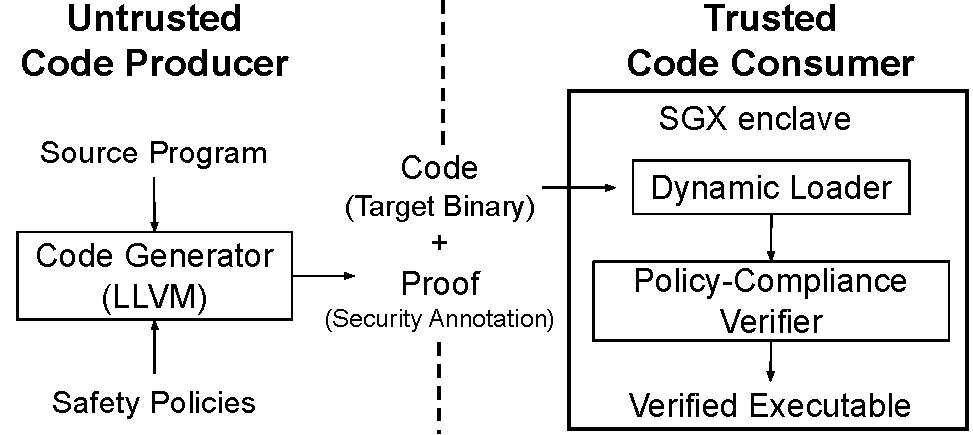
\includegraphics[scale=0.45]{figures/arch_overview.pdf}}
\centerline{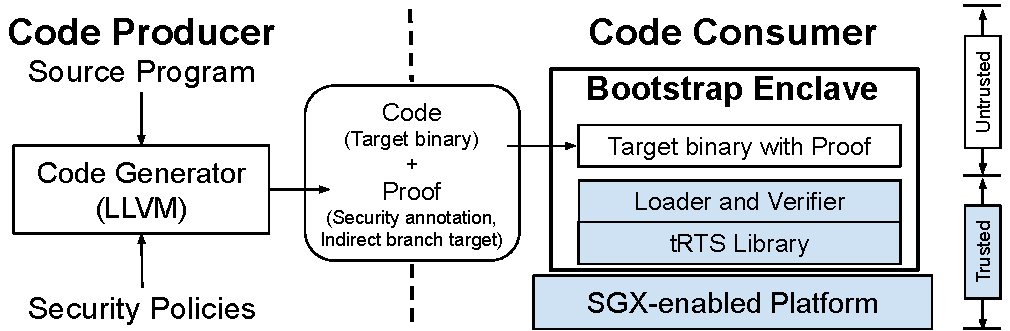
\includegraphics[scale=0.45]{figures/fg-bootstrap-layer.pdf}}
\caption{System overview}\label{fg-overview}
\vspace{-12pt}
\end{figure}

\vspace{3pt}\noindent\textbf{Architecture}. The architecture of is illustrated in Figure~\ref{fg-overview}. The code generator and the binary and proof it produced are all considered untrusted. Only in the TCB is the code consumer with two components: a dynamic-loader operating a rewriter for re-locating the target binary, and a proof verifier running a disassembler for checking the correct instrumentation of security annotations. These components are all made public and can therefore be measured for a remote attestation (Section~\ref{subsec:ra-impl}). They are designed to minimize their code size, by moving most workload to the code producer. 

%\weijie{will unify them all into `verifier'}

%In traditional PCC framework, the VCGen often exists as a compiler~\cite{colby2000certifying,leroy2006formal} or a sandbox~\cite{pirzadeh2010extended}, which is too heavy for limited executive resources. So here, we build our own lightweight PCC system to verify if a cloud service would leakage user’s data. Generally, we provide a code transformer for service code which needs to be verified, and a secure enclave for executing the verified service code. 

%The only TCB in our design is the verifier code inside the enclave, including the dynamic-loader, the disassembler/rewriter (for rewritting structured guards), and the proof verifier (for checking verification hints). On the other hand, the whole trusted code consumer can be remotely attested (in Subsection~\ref{subsec-dynamicloader}), which can indirectly protect the integrity of for code provider, as well as the isolate valuable implementation detail from be accessed.

%As mentioned above, to facilitate PCC framework working well in SGX and to make PCC more efficient, specifically to reduce the size of code consumer side, we move as much proof generation workload as possible to the code producer side, and leave as few verification workload as possible to the inside of the enclave.

\begin{figure*}[htbp]
\centerline{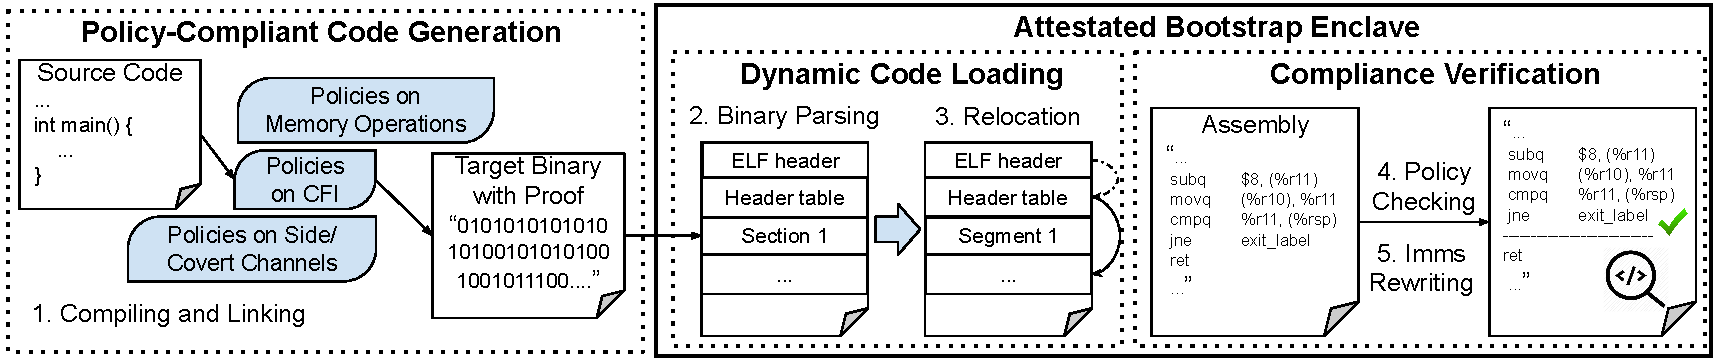
\includegraphics[scale=0.5]{figures/fg-workflow.pdf}}
\caption{Detailed framework and workflow}\label{fg-workflow}
%\wenhao{Typo: Attestated Bootstrap Enclave}
%\weijie{done. Thanks!}
\vspace{-15pt}
\end{figure*}
%\weijie{need some changes on the figure}

 We present the workflow of \textsc{Deflection} in Figure~\ref{fg-workflow}. %Unlike the typical interaction between the producer and consumer, the workflow encompasses several steps. 
The target program (the service code) is first instrumented by the code producer, which runs a customized LLVM-based compiler (step 1). 
%Then on the code consumer side, the loader source code and the verifier source code are compiled with SGX SDK to build the bootstrap enclave binary (step 3). 
Then the target binary with the proof are delivered to the enclave. The code is first parsed (step 2) and then disassembled from the binary's entry along with its control flow traces.
\revise{After that, the proof with the assembly
is relocated and activated by the dynamic loader (step 3), further inspected by the verifier and if correct (step 4) before some immdiates being rewriten (step 5).} Finally, after the bootstrap transfers the execution to the target program, the service begins and policies are checked at runtime.

%\weijie{The description of the steps does not match the steps presented in Figure 3; weird/incorrect sentence construction, typos, inconsistent capitalization of 'Step' (After that, the proof with the assembly inspected by the verifier and if correct (step 3) before some immdiates [sic] being rewriten [sic] (step 4), is further relocated and activated by the dynamic loader (Step 5).}

%Our loader can load and unload code after initialization (step 4), followed by being remote attested (step 5). Moreover, the `code + proof' can be transferred to code consumer where SGX is deployed, waiting for being dynamic loaded and rebased into the enclave (step 6). After being loaded, the verifier will rewrite some key immediate operands (Imm) and finally transfer the execution to the target program (step 7). 

\ignore{
\vspace{3pt}\noindent\textbf{Dynamic Code Loading and Unloading.} \label{subsec-dynamicloader}
%To ensure the bootstrap enclave's code can be completely public and can be attested, we propose a multi-step loader that can load and unload a generated `code + proof' dynamically. Unlike previous work, our proposed solution can resolve the problem that remote attestation conflicts with the dynamic relocation requirement~\cite{seo2017sgx}. Specifically, remote attestation requires code, data and security properties of the enclave to remain unchanged, while executing a private binary code needs relocation for execution, which is a modification to memory distribution. 
%Our proposal is based on the fact that binary code to be verified can not be trusted, so the measurement of the enclave should not include the untrusted code. Therefore, the code to be verified should be dynamically loaded and relocated after the bootstrap enclave is initiated. 
%\weijie{elaborates it later in Section Implementation}
%\vspace{3pt}\noindent\textbf{Separated Linking and Rebasing.} 
In our design, the linking procedures (linking and rebasing) of a target program are separated into both inside and outside the enclave respectively. SGX only accepts that code running inside an enclave is linked against the SGX SDK at build time. For a self-contained function (i.e., one does not use external elements), compiling and sending the bytes of the assembled code is enough. However, if the function uses external elements, a distributed mechanism is needed to map these elements into their corresponding positions at the enclave side. So we use separated linking and rebasing to assemble all the symbols of the entire code (including necessary libraries and dependencies) into one relocatable file (aka. linking), and then parse the symbols and load/relocate the code at runtime inside the enclave (aka. rebasing). Further, during the linkage procedure, we also load and relocate an indirect branch target entry list as part of the proof for later runtime verification.
%Note that legal jump addresses can not be settled until the rebasing procedure is completed because rebasing will modify the addresses of symbols.

The rebasing process starts with the bootstrap enclave receiving the generated binary code through a buffer. The dynamic loader's primary task is to rebase all of its symbols according to information in its relocation table. Therefore, the loader reads relocation tables in the code, updates symbol offsets in its symbol tables, and loads symbols to addresses designated in the relocation table. After rebasing, the detailed memory layout is shown on the right side in Fig.~\ref{fg-dynloader}.
}



%\wenhao{can elaborate on this. The numbers are not in any order}

\subsection{Security Policies}\label{subsec-policies}
%\subsection{Security Policies for the Privacy Preserving Online Data Processing Scenario}\label{subsec-policies}

%Our general goal of defining safety policies is to design a Privacy-preserving TEE prototype on a service-oriented environment for data owner. Here, we make some rules to constrain our design.
Without exposing its code for verification, the target binary needs to be inspected for compliance with security policies by the bootstrap enclave. These policies are meant to protect the privacy of sensitive data, to prevent its unauthorized disclosure. The current design supports following categories. 

%In this scenario, the bootstrap enclave needs to enforce that the data will not be leaked by the untrusted service code, which is not exposed to the data provider. It can be achieved by enforcing several policies as follows. Notably, the policies put some constraints on the service code, yet we make a lot of effort on these constraints to ensure that the code functionality are intact and necessary for the CAT model.

\vspace{3pt}\noindent\textbf {Enclave entry and exit control}. 
\textsc{Deflection} can mediate the content imported to or exported from the enclave, through the ECall and OCall interfaces, for the purposes of reducing the attack surface and controlling information leaks. 
%In CAT’s model, neither the service code nor the infrastructure is under the control of the user, and they may try to steal the user’s secrets by colluding via covert channels.
Another objective here is to mitigate covert channel leaks through the interface between the enclave and the OS, making the attempt to covertly using users’ data to modulate events (e.g., system call arguments, I/O traffic statistics) hard to succeed.
%\weijie{we support multi-use, by cleaning resident data}

%In such service-oriented scenarios, all the bridge functions should be public and attestable for normal use, we should make restrictions on them. The output is to be produced encrypted and the loader must deal with system calls via a trusted Ocall routine. All ECalls/OCalls will be audited and configured correctly by the bootstrap enclave.

\vspace{2pt}\noindent$\bullet$\textit{ P0: Input constraint, output encryption and entropy control}.
We restrict the ECall interfaces to just serving the purposes of uploading data and code, which perform authentication, decryption and optionally input sanitization (or a simple length check). Also only some types of system calls are allowed through OCalls. Particularly, all network communication through OCalls should be encrypted with proper session keys (for the data owner or the code provider). In CCaaS, the data owner can demand that only one OCall (for sending back results to the owner) be allowed. Note that under such control and verification on explicit I/O channels, as well as system call traces and output data sizes, it becomes more difficult for untrusted code to utilize covert channels via software interfaces, such as system call arguments, for exfiltrating content of user’s input outside the enclave.

%\revise{Further, by controlling and verifying explicit I/O channels, as well as system call traces and data sizes, untrusted code cannot use most covert channels via software interfaces, such as sytem call arguments, to communicate bits from the user’s input to the platform.}
%\weijie{how we validate syscall results? verifying the syscall parameters}
%After the Remote Attestation and the session key exchange, messages sent from the bootstrap enclave should be all encrypted. And for security consideration, the bootstrap enclave can only output once during each service, and the output should be the same length to prevent further inference attacks.

\vspace{3pt}\noindent\textbf{Memory leak control}. Information leak can happen through unauthorized write to the memory outside the enclave, which should be prohibited through the code inspection. 

%In order to prevent data leakage during it being processed by a untrusted code provider, we need a verifier to check if this program is prone to write sensitive information from inside enclave to the outside world. 

\vspace{2pt}\noindent$\bullet$\textit{ P1: Preventing explicit out-enclave memory stores}. This policy prevents the target binary from explicit memory writes. It can be enforced by security annotations through mediation on the destination addresses of memory store instructions (such as \texttt{MOV}) to ensure that they are within the enclave address range \texttt{ELRANGE}).
%An enclave has the ability to write data outside of its EPC memory region arbitrarily. Therefore, the major policy is to prevent the untrusted code from copying the data across enclave boundaries. The policy-compliance verifier needs to ensure that the destinations of memory store instructions such as \texttt{MOV} are within the enclave address range (also known as the \texttt{ELRANGE}). %The first thing we should guarantee is no writes onto non-data section. In addition to check various memory write operations caused by instructions like MOV, we need to prevent another register save/spill operations that possibly push some register value to memory space.

\vspace{2pt}\noindent$\bullet$\textit{ P2: Preventing implicit out-enclave memory stores}. Illicit RSP register save/spill operations can also leak sensitive information to the out-enclave memory by pushing a register value to the address specified by the stack pointer, which is prohibited through inspecting the RSP content~\cite{wang2018detect}.  
    %To address this issue, stack operating instructions need be inspected so that the stack pointer never points to memory regions outside the enclave. 
    
\vspace{2pt}\noindent$\bullet$\textit{ P3: Preventing unauthorized change to security-critical data within the bootstrap enclave}. This policy ensures that the security-critical data would never be tampered with by the untrusted code.
%the code never writes to area used by the bootstrap enclave
%reads or writes secrets in the SSA/TCS area to protect the bootstrap enclave and session keys.
%\wenhao{we do not protect read, so it is updated here}

%which is necessary because strong security properties no longer hold if the thread control structure data is used. In this case the verifier needs to ensure that the untrusted code does not tamper with this kind of data structure.
    %\item \textit{P4: does not read from or write to L’s memory}. %\weijie{User's private code does not load from L’s memory. } %\wenhao{auditing memory loads is heavy? We may need to argue the leakage is controlled?}

%\vspace{3pt}\noindent\textbf{Data execution prevention}. The loaded code 

\vspace{2pt}\noindent$\bullet$\textit{ P4: Preventing runtime code modification}. Since the target code is untrusted and loaded into the enclave during its operation, under SGXv1, the code can only be relocated to the pages with \texttt{RWX} properties. So DEP protection should be in place to prevent the target binary from changing itself or uploading other code at runtime. 
%\vspace{3pt}\noindent\textbf{Supporting SGXv2}.
%Our approach currently uses a software DEP since it relies on SGXv1 instructions that does not support dynamically changing page permissions. The design could be simplified with SGXv2 instructions~\cite{mckeen2016intel} since dynamic memory management inside an enclave is allowed and protected in SGXv2 hardware.  

%\wenhao{I think it should be trivial to support SGX2 platforms, but we can talk about how the design could be simplified with SGX2.}
%Allowing applications to modify the set-in-advance page permissions may break the W $\oplus$ X protocol and compromise our DEP plan. However, Intel acclaims that Enclaves will oversee every dynamic memory management and confirm requests from OS before changes take effect~\cite{mckeen2016intel}. Before accessing newly committed pages, the enclave memory manager must accept the EPC allocation performed by the OS. Some inspections could be used at this time point, wherefore to prevent sensitive information from being leaked. The attestation on enclave would also be re-considered when the EPC memory changes dynamically

%P4: Preventing data execution for the RWX region

%A software DEP scheme is needed to prevent the untrusted code from changing the code at runtime.

\vspace{3pt}\noindent\textbf{Control-flow management}. 
%In order to prevent attackers from bypassing our checks, we need do CFI checks on multiple aspects.\todo{on this part}
To ensure that security annotations and other protection cannot be circumvented at runtime, the control flow of the target binary should not be manipulated. For this purpose, the following policy should be enforced:  

%In our PCC-type scheme, the policy-compliance verifier performs static analysis of the untrusted code. It is essential to prevent attackers from dynamically redirecting the control flow at runtime, which may bypass the check performed when the code is initially loaded. In this respect, the following policies need to be enforced. 

\vspace{2pt}\noindent$\bullet$\textit{ P5: Preventing manipulation of indirect branches to violate policies P1 to P4}. This policy is to protect the integrity of the target binary's control flow, so security annotations cannot be bypassed. To this end, we need to mediate all indirect control transfer instructions, including indirect calls and jumps, and return instructions.


%\revise{We not only consider covert channels based on software interfaces like system calls, but also consider side or covert channels based on hardware limitations or execution time.}

\vspace{3pt}\noindent\textbf{AEX based side/covert channel mitigation}. 
In addition to the covert channel through software interfaces like system calls, we further studied the potential to mitigate the covert channel threat through SGX hardware interfaces.
It is well known that SGX's user-land TEE design exposes a large side-channel surface, which cannot be easily eliminated. In the meantime, prior research focuses on the side-channel attacks causing Asynchronous Enclave Exits (AEXs). Examples include the controlled side channel attack~\cite{xu2015controlled} that relies on triggering page faults, and the attacks on L1/L2 caches~\cite{wang2017leaky}, which requires context switches to schedule between the attack thread and the enclave thread, when Hyper-threading is turned off or a co-location test is performed before running the binary~\cite{chen2018racing}. Such protection can be integrated into \textsc{Deflection} to mitigate the side- or covert-channel attacks in this category, closing an important attack surface.
%, even though we cannot eliminate covert threats in general.

%shows that many side-channel attacks cause Asynchronous Enclave Exits (AEXs). Examples include the controlled side channel attack~\cite{xu2015controlled} that relies on triggering page faults, and the attacks on L1/L2 caches~\cite{wang2017leaky}, which requires context switches to schedule between the attack thread and the enclave thread, when Hyper-threading is turned off or a co-location test is performed before running the binary~\cite{chen2018racing}. CAT-SGX is capable of integrating existing solutions to mitigate the side- or covert-channel attacks in this category.  
%\weijie{this policy can also prevent an OS-level attacker controlling an enclave’s address space, therefore protecting data from privileged software to some extend}

%SGX's user-land TEE design exposes a large side-channel surface, which cannot be easily eliminated. In the meantime, prior research shows that many side-channel attacks cause Asynchronous Enclave Exits (AEXs). Examples include the controlled side channel attack~\cite{xu2015controlled} that relies on triggering page faults, and the attacks on L1/L2 caches~\cite{wang2017leaky}, which requires context switches to schedule between the attack thread and the enclave thread, when Hyper-threading is turned off or a co-location test is performed before running the binary~\cite{chen2018racing}. CAT-SGX is capable of integrating existing solutions to mitigate the side- or covert-channel attacks in this category.  


%Side channels are difficult to eliminate and are severe threats to TEEs such as SGX. As shown in previous works, the abnormal AEXs can be used to detect many low-noise side channels within SGX, such as controlled channel attacks~\cite{xu2015controlled}, and same core L1/L2 cache attacks~\cite{chen2018racing}. We are not meant to design new side channel defenses, nevertheless we propose to transplant  existing side channel detecting techniques, which illustrates the generality of the CAT model. 

%Side and covert channels often hide in the normal behaviors during program execution since the logic of service provider’s code would be very complicated. However, side channel prevention is not an easy task. Here we design some alternative policies for side channel mitigation.

%\vspace{2pt}\noindent$\bullet$\textit{ P6: Controlling page fault frequency}.

\vspace{2pt}\noindent$\bullet$\textit{ P6: Controlling the AEX frequency}. The policy requires the total number of the AEX concurrences to keep below a threshold during the whole computation. Once the AEX is found to be too frequent, above the threshold, the execution is terminated to prevent further information leak.

%The policy uses the AEX rate for detecting attempts for side channel attacks. Once an abnormal AEX rate is detected, the enclave execution is terminated to prevent further information leakage.

%\vspace{2pt}\noindent$\bullet$\textit{ Alternative P6: Detecting page faults with TSX support}. 

%\vspace{2pt}\noindent$\bullet$\textit{ Alternative P7: Detecting AEX by monitoring the SSA}.


%\vspace{3pt}\noindent\textbf{Multi-user isolation}. In the presence of multiple data owners, the target program should not expose one owner's data to others. Our current design of CAT-SGX supports a time-sharing setting, where the enclave serves data owners one by one. 

%This policy should be applied to the concurrent situation, in which more than one thread is running inside the enclave, each serving a different owner, as well as the sequential case, where the enclave serves data owners one by one. 

%In the presence of multiple data owners, the target program should not expose one owner's data to others. This policy should be applied to the concurrent situation, in which more than one thread is running inside the enclave, each serving a different owner, as well as the sequential case, where the enclave serves data owners one by one. 
%When protecting in-enclave time-sharing services, a big challenge is to prevent the service program infected by one user from victimizing another user, and the confidentiality of a user’s data left in the enclave to protect it from leaking to the subsequent user receiving the service.

%\weijie{Here we are talking about the multi-user but single-thread case. If we stick on multi-user and multi-threading cases (discussed in Subsec. 8.3), I think we could enforce the following policy:
%For code provider, he/she can specify a max thread number N, and separate its address space to multiple parts such as .data1 .data2 ... .dataN, for several threads' address space (using different offsets to distinguish those threads' space). 
%For the bootstrap enclave, it will copy the data (from data owner, via an Ecall) to every .dataX section. When performing context switch, firstly it  needs to check that a thread must read/write its own reserved space (e.g., thread1 can only read/write .data1, thread2 can only read/write .data2); secondly, the bootstrap enclave must clear all critical TCS/SSA/TLS when context switching.
%}


%\vspace{2pt}\noindent$\bullet$\textit{ P8: Cleansing data at user switch}. The policy ensures that once the task for one data owner ends, all her data will be removed from the enclave before the next owner's data is loaded into the enclave. \weijie{this part and the multi-user isolation parts mentioned above can be moved to the discussion section}

%The purpose of the data cleansing and the exit sanitization is to reset the service state and clean up the old user’s data right after execution is done. Except the persistent data of the user, all other data will be cleaned up, together with the content of SSA and registers.

\subsection{Policy-Compliant Code Generation}
\label{subsec-producer}

As mentioned earlier, the design of \textsc{Deflection} is to move the workload from in-enclave verification to out-enclave generation of policy-compliant binary and its proof. 
%Since the verification could be done very easily by checking if the policy-compliant proof exists, the essential part of policy enforcement would be how we generate proof-carrying code.
In this section we describe the design of the code generator, particularly how it analyzes and instruments the target program so that security policies (P1-P6, see Section~\ref{subsec-policies}) can be enforced during the program's runtime. Customized policies for purposes other than privacy can also be translated into proof and be enforced flexibly, e.g., to verify code logic and its functionalities.

%\weijie{1. the generated code/instrumentation should be formally proved to be consistant with the policy/in structured format}
%\weijie{2. the verifier should be able to verify the correctness of the instrumentations}
%\weijie{3. definition of correctness: the integrity of instrumentations }
%\weijie{Theorem}
%\weijie{proof. The execution of each instruction $i$ can be represented by a Hoare triple.}

%\weijie{show component/policy flexibility}
%which given the source program can produce binary code with proof that enforces flexible policies and can be verified easily. We enforce each policy strictly according to the security suggestions~\ref{subsec-policies} from P0 to P6. The design of the policy verifier will be presented later in Sec.~\ref{subsec:verify}. 


%When the target binary wants a syscall or the in-enclave service ends, the computing results need to be output in a standard format.
 
% stubs/proxies
%Before that, to construct the output, the messages are padded to a constant length.  
%On the other hand, 37 common system calls are also wrapped with Ocall stubs for possible system interactions. Meanwhile, the output functions are wrapped by our customized Ocall stubs.


%In scenarios like serving an HTTPS server and other network services, only the send/receive Ocall interfaces are allowed, and the interval time of each send/receive can be padded to prevent the timing covert channels.
%\wenhao{do we implement the fixed time scheme for https server? if we say it here, it may needed to be evaluated}
%\weijie{we donot implement the fixed time currently}
%\weijie{The output length of an Ocall is fixed, for scenario 2.}\weijie{we have to ack we only limited some side channel/covert channels.}


%enforcing mem ops
\vspace{3pt}\noindent\textbf{Enforcing P1}.  The code generator is built on top of the LLVM compiler framework (Section~\ref{subsec-instrument}). When compiling the target program (in C) into binary, the code generator identifies (through the LLVM API \verb|MachineInstr::mayStore()|) all memory storing operation instructions (e.g., \texttt{MOV}, Scale-Index-Base (SIB) instructions) and further inserts annotation code before each instruction to check its destination address and ensure that it does not write outside the enclave at runtime. 
The boundaries of the enclave address space can be obtained during dynamic code loading, which is provided by the loader (Section~\ref{subsec:verify}). The correct instrumentation of the annotation is later verified by the code consumer inside the enclave. 

%The code consumer the enclave confirms such security check instructions are in place.

\vspace{3pt}\noindent\textbf{Enforcing P2}. 
%The generator prevents implicit memory write crossing the enclave boundaries by making sure the stack pointer never point to memory regions outside the enclave. 
The generator locates all instructions that explicitly modify the stack pointer (the RSP in x86 arch) from the binary (e.g., a \texttt{MOV} changing its content) and inserts annotations to check the validity of the stack pointer after them. This protection, including the content of the annotations and their placement, is verified by the code consummer (Section~\ref{subsec-loading}). 
Note that RSP can also be changed implicitly, e.g., through pushing oversized objects onto the stack. This violation is prevented by the loader (Section~\ref{subsec-loading}), which adds guard pages (pages without permission) around the stack. 

%Furthermore, the code consumer prevents implicit modification (pushing oversized objects to the stack) to the stack pointer by adding guard pages (i.e., pages granted no permissions) around the stack boundaries. 

\vspace{3pt}\noindent\textbf{Enforcing P3}. Similar to the enforcement of P1 and P2, the code generator inserts security annotations to prevent (both explicit and implicit) memory write operations on security-critical enclave data (e.g., SSA/TLS/TCS) once the untrusted code is loaded and verified. 
%These annotation instructions are verified later by the verifier. 

%enforcing DEP
\vspace{3pt}\noindent\textbf{Enforcing P4}. To prevent the target binary from changing its own code at runtime, the code generator instruments all its write operations (as identified by the APIs \verb|readsWritesVirtualRegister()| and \verb|mayStore()|) with the annotations that disallow alternation of code pages. Note that the code of the target binary has to be placed on \texttt{RWX} pages by the loader under SGXv1 and its stack and heap are assigned to \texttt{RW} pages (see Sec.~\ref{subsec-loading}), so runtime code modification cannot be stopped solely by page-level protection (though code execution from the data region is defeated by the page permissions). 
%\weijie{SGXv2 based DEP}

%\weijie{We loaded the code segment on the RWX pages and the data segment on the RW pages.}
%Similar to the enforcement of P1 and P2, the code generator instruments the binary to ensure that memory write operations cannot write any content on the \texttt{RWX} pages, which is only generated for target code loading (detailed in Sec.~\ref{subsec-dynamicloader}). 
%We can combine the enforcement of from P1 to P4, setting several boundaries for all of them.

%enforcing CFI
\vspace{3pt}\noindent\textbf{Enforcing P5}. To control indirect calls or indirect jumps in the target program, the code generator extracts all labels from its binary during compilation and instruments security annotations before related instructions to ensure that only these labels can serve as legitimate jump targets. The locations of these labels should not allow an instrumented security annotations to be bypassed. 
Also to prevent the backward-edge control flow manipulation (through \texttt{RET}), the generator injects annotations after entry into and before return from every function call to operate on a shadow stack, which is allocated during code loading. Also all the legitimate labels are replaced by the loader when relocating the target binary. Such annotations are then inspected by the verifier when disassembling the binary to ensure that protection will not be circumvented by control-flow manipulation (Section~\ref{subsec-disassembling}).  



%Then the loader transforms them to legal destination addresses, and stores them as a list in a specific reserved region. 

%It instruments code to check the targets of all indirect call/jump instructions in the code to ensure they only direct to addresses on that list. 

%A shadow stack is also included, to prevent backward-edge control flow manipulation.


%Instruments can be efficiently verified, while the integrity of the indirect branches will be checked during disassembling (Section~\ref{subsec-disassembling}).

%\weijie{the (loader and verifier) will check the following 3 things:}
%\yaosong{}

%0. the (loader and verifier) finds (and verifies) all legal targets according to the given list;

%1. instrumentations (for indirect branches and ret instructions) are in place and in correct formats;

%2. the targets of direct branches are not between the original code and the instrumentation;


%enforcing side channel mitigations

%\vspace{3pt}\noindent\textbf{Enforcing P6 with TSX (P6-TSX)}. To mitigate AEX based side-channel risks, CAT-SGX provides two enforcement mechanisms, through TSX or SSA inspection, which can be chosen when compiling the target program. The TSX approach is based upon T-SGX~\cite{shih2017t}, putting transaction memory protection on each basic block and running a fall-back function to keep track of the number of interrupts observed. When more than XX consecutive AEXes happen, the computation aborts, due to the concern of an ongoing side-channel attack.  The protection is instrumented by the generator and its presence is verified by the code consumer in the enclave. 
%\xiaofeng{Remove the above paragraph?}

%which isolates the fallback handler and other transaction control code, called springboard, from the original program’s code and data pages to ensure that exceptions such as page faults and timer interrupts can only be triggered on the springboard. We take advantage of it and implement instruction wrappers that encompass all boundaries between any basic blocks and branches. The fallback route of the TSX wrapper records the number of transaction aborts, which ensures that if a threshold is exceeded, the program is forced to exit. 

%\weijie{up to 10 consecutive transaction aborts are allowed for each individual basic block} We enforce P6 by introducing the idea of T-SGX~\cite{shih2017t}. As a compiler-level scheme that automatically transforms a normal enclave program into a secured one, T-SGX can isolate the fallback handler and other transaction control code, called springboard, from the original program’s code and data pages to ensure that exceptions including page faults and timer interrupts can only be triggered on the springboard. We take advantage of it and implement instruction wrappers that encompass all boundaries between any basic blocks and branches. The fallback route of the TSX wrapper records the number of transaction aborts, which ensures that if a threshold is exceeded, the program is forced to exit. 


\vspace{3pt}\noindent\textbf{Enforcing P6 with SSA inspection}. When an exception or interrupt take place during enclave execution, an AEX is triggered by the hardware to save the enclave context (such as general registers) to the state saving area (SSA). This makes the occurrence of the AEX visible~\cite{gruss2017strong,chen2018racing}. Specifically, the code generator enforce the policy by instrumenting every basic block with an annotation that sets a marker in the SSA and monitors whether the marker is overwritten, which happens when the enclave context in the area has been changed, indicating that an AEX has occurred. Through counting the number of consecutive AEXes, the protected target binary can be aborted in the presence of anomalously frequent interrupts. This protection is verified by the code consumer before the binary is allowed to run inside the enclave. 


\vspace{3pt}\noindent\textbf{Code loading support}.\label{subsec:code-loading-support}
Loading the binary is a procedure that links the binary to external libraries and relocates the code. 
For a self-contained function (i.e., one does not use external elements), compiling and sending the bytes of the assembled code is enough. However, if the function wants to use external elements but not supported inside an enclave (e.g., a system call), a distributed code loading support mechanism is needed. In our design, the loading procedure is divided into two parts, one (linking) outside and the other (relocation) inside the enclave.
%Specifically, SGX only accepts that code running inside an enclave is linked with the SGX SDK at build time.
Our code generator assembles all the symbols of the entire code (including necessary libraries and dependencies) into one relocatable file via static linking. While linking all object files generated by the LLVM, it keeps all symbols and relocation information held in relocatable entries. 
%(offset values that denoted within a section header, in which the relocations have to take place).
The relocatable file, as above-mentioned target binary, is expected to be loaded for being relocated later (Section~\ref{subsec-loading}).

%parse the symbols and map these elements into their corresponding positions at the enclave side later. 

%%%%%%%%%%%%%%%%%%%%%%%%%%%%%%%%%%%%%%%%%%%%%%%

%The execution is terminated once the number of AEXs within the basic block exceeds a preset threshold.

%When an exception or interrupt is triggered during the enclave execution, the AEX performed by the hardware saves the enclave context (such as general registers) to the state saving area (SSA). As demonstrated in previous works~\cite{gruss2017strong,chen2018racing}, AEX can be detected by monitoring the SSA. We instrument every basic block to set a marker in the SSA and monitor whether the marker is overwritten by AEX within the basic block. The execution is terminated once the number of AEXs within the basic block exceeds a preset threshold.

%Another by retrofitting Hyperrace~\cite{chen2018racing}. However, unlike Hyperrace doing the physical-core co-location tests, here we only monitor how often the interrupts/AEXs happen. L1/L2 cache-based channel can be detected when certain number or more interrupts/AEXs occur in one basic block or every $k$ instructions.

%enforcing multi-user isolation
%\vspace{3pt}\noindent\textbf{Enforcing P8}. Before the in-enclave is finished, all user data is cleared.


\subsection{Configuration, Loading and Verification}
\label{subsec:verify}

With annotations instrumented and legitimate jump targets identified, the in-enclave workload undertaken by the bootstrap enclave side has been significantly reduced. Still, it needs to be properly configured to enforce the policy (P0) that cannot be implemented by the code generator.
%, load and relocate the target binary so instrumented protection can be properly executed and also verify the ``proof'' for policy compliance through efficient dissembling and inspecting the binary. 
Following we elaborate how these critical operations are supported by our design.   


%Due to the thorough generated proof with compliance, the bootstrap enclave can quickly verify the validity of the proof, and it can compare the conclusions of the proof to its own security policy to determine whether the application is safe to execute.

\vspace{3pt}\noindent\textbf{Enclave configuration to enforce P0}. 
To enforce the input constraint, we need to configure the enclave by defining certain public ECalls in Enclave Definition Language (EDL) files for data and code secure delivery. Note such a configuration, together with other security settings, can be attested to the remote data owner or code provider. The computation result of the in-enclave service is encrypted using a shared session key after the remote attestation and is sent out through a customized OCall. For this purpose, \textsc{Deflection} only defines allowed system calls (e.g., \texttt{send/recv}) in the EDL file, together with their wrappers for security control (e.g., verifying the system call arguments).
To support the basic CCaaS setting,  \texttt{send} and \texttt{recv} need to be communicated to the data owner.  
Specially, the wrapper for \texttt{send} encrypts the message to be delivered and pads it to a fixed length. For more complicated settings, we only permit a list of OCalls to be invoked once to deliver the computing result to the code provider, which can be enforced by the wrapper of the function. Further the wrapper can put a constraint on the length of the result to control the amount of information disclosed to the code provider: e.g., only 8 bits can be sent out. 

%\revise{the basic CCaaS setting,  \texttt{send} and \texttt{recv} must be allowed to communicate with the data owner.  Specially, the wrapper for \texttt{send} encrypts the message to be delivered and pads it to a fixed length. For more complex settings, we only permit a list of OCalls}
%When necessary, the wrappers of these functions can pad the encrypted output and ensure that the inter-packet timings are constant to mitigate the covert-channel risk.

\vspace{3pt}\noindent\textbf{Dynamic code loading and unloading}. \label{subsec-loading}
%To ensure the bootstrap enclave's code can be completely public and can be attested, we propose a multi-step loader that can load and unload a generated `code + proof' dynamically. Unlike previous work, our proposed solution can resolve the problem that remote attestation conflicts with the dynamic relocation requirement~\cite{seo2017sgx}. Specifically, remote attestation requires code, data and security properties of the enclave to remain unchanged, while executing a private binary code needs relocation for execution, which is a modification to memory distribution. 
%Our proposal is based on the fact that binary code to be verified can not be trusted, so the measurement of the enclave should not include the untrusted code. Therefore, the code to be verified should be dynamically loaded and relocated after the bootstrap enclave is initiated. 
%\weijie{elaborates it later in Section Implementation}
%\vspace{3pt}\noindent\textbf{Separated Linking and Rebasing.} 
The target binary is delivered into the enclave as data through an ECall, processed by the wrapper placed by \textsc{Deflection}, which authenticates the sender and then decrypts the code before handing it over to the dynamic loader. The primary task of the loader is to rebase all symbols of the binary according to its relocation information (Section~\ref{subsec:code-loading-support}). For this purpose, the loader first parses the binary to retrieve its relocation tables,  then updates symbol offsets\ignore{ based upon the symbol tables}, and further reloads the symbols to designated addresses. During this loading procedure, the indirect branch label list is ``translated'' to in-enclave addresses, which are considered to be legitimate branch targets and later used for policy compliance verification. 

%Note that legal jump addresses can not be settled until the rebasing procedure is completed because rebasing will modify the addresses of symbols.
%The rebasing process starts with the bootstrap enclave receiving the generated target binary code through a buffer. The dynamic loader's primary task is to rebase all of its symbols according to the information in its relocation table. Therefore, the loader reads relocation tables of the binary, updates symbol offsets of its symbol tables, and reloads symbols to designated addresses. During the loading procedure, the indirect branch label list is also loaded as part of the proof for later verification.

As mentioned earlier (Section~\ref{subsec-producer}), the code section of the target binary is placed on pages with \texttt{RWX} privileges, since under SGXv1, the page permissions cannot be changed during an enclave's operation, while the data sessions (stack, heap) are assigned to the pages with \texttt{RW} privileges. These code pages for the binary are guarded against any write operation by the annotations for enforcing P4. Other enclave code, including that of the code consumer, is under the \texttt{RX} protection through enclave configuration. Further the loader assigns two non-writable blank guard pages right before and after the target binary's stack for enforcing P2, and also reserves pages for hosting the list of legitimate branch targets and the shadow stack for enforcing P5. 


%To facilitate the policy enforcement as described in Section~\ref{subsec-producer}, all sections are allocated with either \texttt{RX} or \texttt{RW} privileges, except the memory buffer \texttt{RWX} reserved for target binary delivery, which however can be protected by our data execution prevention enforcement (P4). 
%The loader also provides two non-writable blank guard pages right before and after the target code stack (for enforcing P2). Moreover, our loader resolves the targets from labels to legal addresses, and reserves a branch target list region and a shadow stack space (for enforcing P5). 
%After rebasing, the detailed memory layout is shown on the right side in Fig.~\ref{fg-dynloader}.


%\weijie{no SGX1/2 instructions}

\vspace{3pt}\noindent\textbf{Just-enough disassembling and verification}.
\label{subsec-disassembling} After loading and relocating, the target binary is passed to the verifier for a policy compliance check. Such a verification is meant to be highly efficient, together with a lightweight disassembler. Specifically, our disassembler is designed to leverage the assistance provided by the code generator.  It starts from the program entry discovered by the parser and follows its control flow until an indirect control flow transfer, such as indirect jump or call, is encountered. Then, it utilizes all the legitimate target addresses on the list to continue the disassembly and control-flow inspection. In this way, the whole program will be quickly and comprehensively examined.  

%\revise{In particular, verification states model register contents, including the contents of the shadow stack which holds function-local virtual registers.}
For each indirect branch, the verifier checks the annotation code (Figure~\ref{subsec-producer}) right before the branch operation, which ensures that the target is always on the list at runtime. Also, these target addresses, together with direct branch targets, are compared with all guarded operations in the code to detect any attempt to evade security annotations. To simplify the verification of the CFI policy compliance, the verifier utilizes \textit{hints} (i.e., the symbol  name on the list) to identify the set of possible targets for calls/jumps. For this purpose, the verifier scans the machine code  to ensure that these identifiers appear only at the beginning of basic blocks. The verification of P6 for covert channel mitigation is done one basic block at a time, and on the basic-block exit the verifier checks whether all policy-compliance instrumentations are in position at the entries to all possible successor blocks.

%\revise{To simplify the verification of the CFI policy compliance, the verifier expects hints (aka. the symbol  name on the list) to specify the set of possible targets of calls/jumps. The verifier scans the machine code in order to ensure that these identifiers occur only at the beginning of basic blocks.}

With such verification, no hidden control transfers will be performed by the binary, allowing further inspection of other instrumented annotations. These annotations are expected to be well formatted and located around the critical operations as described in Section~\ref{subsec-producer}. %Figure~\ref{fg-mov} presents an example. 
More details are given in Section~\ref{subsec-instrument} and our Github repository~\cite{our-prototype}.


%\revise{Figure~\ref{} shows an example on memory inline guards.Figure~\ref{} shows an example on CFI inline guards.Figure~\ref{} shows an example on shadow stack inline guards.}

%the target is on the list. Also all direct or indirect branches discovered  . When we encounter indirect control flow transfers such as indirect jumps and indirect calls, we use the valid target list provided to find the targets of indirect control flows. Note that our verifier will ensure that there are runtime checks before every indirect control flow, which guarantees that the actual control flow targets are inside the list provided by the compiler. When jumping to next target, we check if the targets will not be inside any instrumentations.
%enforced by policies (in Section~\ref{subsec-producer}).

%In this way, the untrusted compiler is not able to hide dangerous transfer targets by omitting them in the list. Finally, the instrumentations executed at runtime will guarantee that the CFI (P5) of the target program is enforced.     


%To ensure compliance with other policies, the verifier checks whether the instrumented annotations are in place and in structured format. More examples can be found at section implementation and appendix.


%Accurate and complete binary disassembly is a difficult problem in general due to indirect control flow transfers. We built a lightweight disassembler with the assistance of the compiler outside the enclave. Our disassembler starts with the program entry and follows the program control flow. When we encounter indirect control flow transfers such as indirect jumps and indirect calls, we use the valid target list provided to find the targets of indirect control flows. Note that our verifier will ensure that there are runtime checks before every indirect control flow, which guarantees that the actual control flow targets are inside the list provided by the compiler. 
%When jumping to next target, we check if the targets will not be inside any instrumentations.
%enforced by policies (in Section~\ref{subsec-producer}).
%In this way, the untrusted compiler is not able to hide dangerous transfer targets by omitting them in the list. Finally, the instrumentations executed at runtime will guarantee that the CFI (P5) of the target program is enforced. 
%To ensure compliance with other policies, the verifier checks whether the instrumented annotations are in place and in structured format. More examples can be found at section implementation and appendix.




%Accurate and complete binary disassembly is a difficult problem in general due to indirect control flow transfers. We built a lightweight disassembler with the assistance of the compiler outside the enclave. Our disassembler starts with the program entry and follows the program control flow. When we encounter indirect control flow transfers such as indirect jumps and indirect calls, we use the valid target list provided to find the targets of indirect control flows. Note that our verifier will ensure that there are runtime checks before every indirect control flow, which guarantees that the actual control flow targets are inside the list provided by the compiler. When jumping to next target, we check if the targets will not be inside any instrumentations.
%enforced by policies (in Section~\ref{subsec-producer}).
%In this way, the untrusted compiler is not able to hide dangerous transfer targets by omitting them in the list. Finally, the instrumentations executed at runtime will guarantee that the CFI (P5) of the target program is enforced. 
%\vspace{3pt}\noindent\textbf{Leveraging Intel MPX and Bnd Instructions.} Recent work shows that Intel MPX can coroperate well with Intel SGX for boundary checking~\cite{shen2018isolate}~\cite{kuvaiskii2017sgxbounds}. Simple instructions like BNDCL and BNDCU could be instrumented where we check the target address with lower and upper memory bounds. In CAT, we leverage this hardware feature as well. Yet this part is under construction and we believe that it will boost the performance of policy checking part of our system.



%-------------------------------------------------------------------------------------------







\ignore{

\vspace{3pt}\noindent\textbf{Enforcing P0}. 
To enforce the input constraint, we define certain public ECalls in Enclave Definition Language (EDL) files for data and code secret delivery, which can be attested by the remote data owner.
The computation result of the in-enclave service is encrypted using session key after RA and will be output in a customized OCall. Before that, to construct the output, the messages are padded to a constant length.  
%On the other hand, 37 common system calls are also wrapped with Ocall stubs for possible system interactions. Meanwhile, the output functions are wrapped by our customized Ocall stubs.
In this CCaaS setting, only one Ocall (for outputing the computation result) is allowed to execute once. In scenarios like serving an HTTPS server and other network services, only the send/receive Ocall interfaces are allowed, and the interval time of each send/receive can be padded to prevent the timing covert channels.
%\wenhao{do we implement the fixed time scheme for https server? if we say it here, it may needed to be evaluated}
%\weijie{we donot implement the fixed time currently}
%\weijie{The output length of an Ocall is fixed, for scenario 2.}\weijie{we have to ack we only limited some side channel/covert channels.}


%enforcing mem ops
\vspace{3pt}\noindent\textbf{Enforcing P1}. The code generator finds all memory storing operations and instruments annotation code before them to make sure they are writing to the address space out of the enclave. 
The boundaries of the enclave address space can be obtained during the procedure of dynamic code loading (Sec.~\ref{subsec:verify}).
The code consumer the enclave confirms such security check instructions are in place.

\vspace{3pt}\noindent\textbf{Enforcing P2}. 
%The generator prevents implicit memory write crossing the enclave boundaries by making sure the stack pointer never point to memory regions outside the enclave. 
The generator locates all the instructions modifying the stack pointer (aka. the RSP in x86 arch) explicitly, and inserts instructions to check the validity of the stack pointer after them. The code consumer confirms the placement of these check instruction. Furthermore, the code consumer prevents implicit modification (pushing oversized objects to the stack) to the stack pointer by adding guard pages (i.e., pages granted no permissions) around the stack boundaries. 

\vspace{3pt}\noindent\textbf{Enforcing P3}. Similar to enforcing P1 and P2, the code generator further enforces that (both explicit and implicit) memory write operations cannot alter the security-critical data once the untrusted code is loaded and verified. These annotation instructions are verified later in the verifier. 

%enforcing CFI
\vspace{3pt}\noindent\textbf{Enforcing P4}. Similar to enforcing P1 and P2, the code generator and consumer enforce that memory write operations cannot modify the \texttt{RWX} pages. We can combine the enforcement of from P1 to P4, setting several boundaries for all of them.

\vspace{3pt}\noindent\textbf{Enforcing P5}. For indirect calls or indirect jumps, the code generator firstly extract all legal destination addresses, then store them as a list in a specific reserved region. It instruments code to check the targets of all indirect call/jump instructions in the code to ensure they only direct to addresses on that list. A shadow stack is also included, to prevent backward-edge control flow manipulation.
Instruments can be efficiently verified, while the integrity of the forward-edge indirect branches will be checked during disassembling (Section~\ref{subsec-disassembling}).

%enforcing side channel mitigations

\vspace{3pt}\noindent\textbf{Enforcing P6 by detecting page faults with TSX support (P6-TSX)}.
%\weijie{up to 10 consecutive transaction aborts are allowed for each individual basic block}
We enforce P6 by introducing the idea of T-SGX~\cite{shih2017t}. As a compiler-level scheme that automatically transforms a normal enclave program into a secured one, T-SGX can isolate the fallback handler and other transaction control code, called springboard, from the original program’s code and data pages to ensure that exceptions including page faults and timer interrupts can only be triggered on the springboard. We take advantage of it and implement instruction wrappers that encompass all boundaries between any basic blocks and branches. The fallback route of the TSX wrapper records the number of transaction aborts, which ensures that if a threshold is exceeded, the program is forced to exit. 

\vspace{3pt}\noindent\textbf{Enforcing P6 by detecting AEX with monitoring the SSA (P6-SSA)}. When an exception or interrupt is triggered during the enclave execution, the AEX performed by the hardware saves the enclave context (such as general registers) to the state saving area (SSA).
As demonstrated in previous works~\cite{gruss2017strong,chen2018racing}, AEX can be detected by monitoring the SSA. We instrument every basic block to set a marker in the SSA and monitor whether the marker is overwritten by AEX within the basic block. The execution is terminated once the number of AEXs within the basic block exceeds a preset threshold.
%Another by retrofitting Hyperrace~\cite{chen2018racing}. However, unlike Hyperrace doing the physical-core co-location tests, here we only monitor how often the interrupts/AEXs happen. L1/L2 cache-based channel can be detected when certain number or more interrupts/AEXs occur in one basic block or every $k$ instructions.

%enforcing multi-user isolation
%\vspace{3pt}\noindent\textbf{Enforcing P8}. Before the in-enclave is finished, all user data is cleared.


\subsection{Code Loading and Compliance Verification}
\label{subsec:verify}

Due to the thorough generated proof with compliance, the bootstrap enclave can quickly verify the validity of the proof, and it can compare the conclusions of the proof to its own security policy to determine whether the application is safe to execute.

\vspace{3pt}\noindent\textbf{Dynamic code loading and unloading}. \label{subsec-dynamicloader}
%To ensure the bootstrap enclave's code can be completely public and can be attested, we propose a multi-step loader that can load and unload a generated `code + proof' dynamically. Unlike previous work, our proposed solution can resolve the problem that remote attestation conflicts with the dynamic relocation requirement~\cite{seo2017sgx}. Specifically, remote attestation requires code, data and security properties of the enclave to remain unchanged, while executing a private binary code needs relocation for execution, which is a modification to memory distribution. 
%Our proposal is based on the fact that binary code to be verified can not be trusted, so the measurement of the enclave should not include the untrusted code. Therefore, the code to be verified should be dynamically loaded and relocated after the bootstrap enclave is initiated. 
%\weijie{elaborates it later in Section Implementation}
%\vspace{3pt}\noindent\textbf{Separated Linking and Rebasing.} 
In our design, the linking procedures (linking and rebasing) of a target program are separated into both inside and outside the enclave respectively. SGX only accepts that code running inside an enclave is linked against the SGX SDK at build time. For a self-contained function (i.e., one does not use external elements), compiling and sending the bytes of the assembled code is enough. However, if the function uses external elements, a distributed mechanism is needed to map these elements into their corresponding positions at the enclave side. So we use separated linking and rebasing to assemble all the symbols of the entire code (including necessary libraries and dependencies) into one relocatable file (aka. linking), and then parse the symbols and load/relocate the code at runtime inside the enclave (aka. rebasing). Further, during the linkage procedure, we also load and relocate an indirect branch target entry list as part of the proof for later runtime verification.
%Note that legal jump addresses can not be settled until the rebasing procedure is completed because rebasing will modify the addresses of symbols.

The rebasing process starts with the bootstrap enclave receiving the generated target binary code through a buffer. The dynamic loader's primary task is to rebase all of its symbols according to the information in its relocation table. Therefore, the loader reads relocation tables of the binary, updates symbol offsets of its symbol tables, and reloads symbols to designated addresses. 
%After rebasing, the detailed memory layout is shown on the right side in Fig.~\ref{fg-dynloader}.


\vspace{3pt}\noindent\textbf{Just-enough disassembling and verification}.
\label{subsec-disassembling}
Accurate and complete binary disassembly is a difficult problem in general due to indirect control flow transfers. We built a lightweight disassembler with the assistance of the compiler outside the enclave. Our disassembler starts with the program entry and follows the program control flow. When we encounter indirect control flow transfers such as indirect jumps and indirect calls, we use the valid target list provided by the compiler to find the targets of indirect control flows. Note that our verifier will ensure that there are runtime checks before every indirect control flow, which guarantees that the actual control flow targets are inside the list provided by the compiler. 
When jumping to next target, we check if the target is inside any instrumentations enforced by policies (in Section~\ref{subsec-producer}).
In this way, the untrusted compiler is not able to hide dangerous transfer targets by omitting them in the list. The runtime check ensures the integrity of the target list provided by the compiler. 


}








\ignore{


As described in Sec.~\ref{sec-CAT}, a confidential attestation process encompasses a standard Intel attestation to attest the bootstrap enclave and establish a secure communication channel. If they are convinced that the bootstrap enclave can enforce the desired security policies, the data or code providers can send the data and code (in encrypted form) to the bootstrap enclave. 

In this section we present our design for realizing the CAT model under the privacy preserving data processing scenario. In this setting, the service user (i.e., the data owner) communicates with the remote data processing service with encrypted messages for uploading her data and receiving the results.
%sends and receives  from remote parties. The service provider is with the infrastructure's side so that the code can be conveyed directly into the bootstrap enclave. 
To minimize the size of the bootstrap enclave, the design borrows the idea of PCC and consists of an untrusted code producer outside the enclave, and a trusted code consumer inside.
Sec.~\ref{subsec-threat} presents the threat model. Sec.~\ref{subsec-policies} presents the categorized security policies enforced by the bootstrap enclave. Sec.~\ref{subsec-producer} and Sec.~\ref{subsec:verify} presents how the policies can be enforced and verified with the cooperative design of the code producer and code consumer.
We will discuss how to extend the design to other scenarios with carefully crafted security policies in Sec.~\ref{subsec:morescenario}. 


%with little or no modification since the code generator and the policy-compliance verifier can work perfectly independently and have no impact on one another.

%-----------------------------------------

\ignore{
\subsection{Threat model}
\label{subsec-threat}
%In this paper we assume a strong adversary in the CAT model, i.e., the code providers and data providers do not trust each other. 
To demonstrate how to instantiate the CAT model, in the rest of the paper we consider a specific application scenario, i.e., privacy preserving online data processing (Scenario 1 in Sec.~\ref{subsec-scenarios}). As shown in Sec.~\ref{subsec-motivation}, many real world privacy preserving data processing tasks fall into this scenario. 
%We stress that instantiating the CAT model in the other application scenarios are important future works.
As described earlier for Scenario 1, the user (i.e., the data provider) submits her sensitive data to a service provider (i.e., the code owner) for data processing tasks. In our threat model, we make the following assumptions.
 
%Before the discussion of how we design a practical Privacy-preserving TEE, a threat model could be built for better define the scope of the problem we need to solve. 

\vspace{2pt}\noindent$\bullet${ The service code and the SGX-enabled host platform are not trusted.} The service provider may (intentionally) write vulnerable service code which causes the leakage of the users' data.
%, e.g., the enclave may be compromised by another user with memory corruption attacks. 
The service code can even collude with the SGX-enabled platform owned and controlled by the attacker, e.g., through covert channels (such as page faults etc.). 

%to do whatever they can to steal the data owner’s sensitive information. But we believe in Intel SGX and its RA protocol, which could be seen as a trusted third party.

%\weijie{The data provider is relatively benign and won't do anything to jeopardize the code privacy, e.g., sending some malicious input (triggering unexpected attacks) into the code. }
%\hongbo{Do we need to mention the cloud computation platform is also untrusted?}
\vspace{2pt}\noindent$\bullet$ Since the service provider is untrusted, our design does not intend to guarantee the correctness of the results returned to the users. The service users can refuse to pay for the service or turn to other service providers if the results are inferior. This is similar as Denial-of-Service (DoS) attacks which are also out of scope.

\vspace{2pt}\noindent$\bullet$ Besides, we assume the bootstrap enclave code can be inspected (or formally verified) by the users through remote attestation, so that it is trusted to be functional as designed. We trust the SGX hardware and the Intel's attestation protocol as well as the cryptographic algorithms underneath. The mutual authentication between the users and service provider is orthogonal to the design and is omitted in the paper.

%\vspace{2pt}\noindent$\bullet$\textit{The data is encrypted and intact before the enclave starts to run the data-processing application.} Intel SGX and its built-in toolsets can make both the service provider’s code and user’s data loaded into an enclave securely via RA and key exchange. And if necessary, service provider could apply some differential privacy techniques and add certain noisy to protect the data from inference attacks.
    %As discussed earlier the loaded code cannot perform Ocalls directly, and we assume that all ECalls/OCalls will be audited by the bootstrap enclave. 
    %Since all the bridge functions should be public for normal use, it makes sense that we can make such assumption in this service-oriented scenarios. And if necessary, service provider could add certain noisy to protect the data from inference attacks.
    %\item Currently, we do not consider side channels or covert channels between the enclave code and the outside world. In this paper, we are confined to verifying simple confidentiality properties and do not handle complex adversary models like those involving side-channels.\wenhao{remove this item}

}


%------------------------------------------------------------------------


\subsection{CAT-SGX: Overview}
\label{subsec-overview}

A common method to enable efficient verification of the code properties within the bootstrap enclave is to use PCC. We find, however, applying traditional PCC schemes directly to the CAT model is impractical due to the following reasons: (1) Traditional PCC schemes induce huge TCB, including the VC generator with an intermediate  language interpreter/compiler, or a virtual machine that can support runtime proof checking. (2) In traditional PCC schemes, the proof size is usually large. (3) Although the procedure of generating proof runs outside the enclave and is not trusted, it usually takes exponential time with respect to the code size and may take too long for real world data processing computations.

\begin{figure}[htbp]
%\centerline{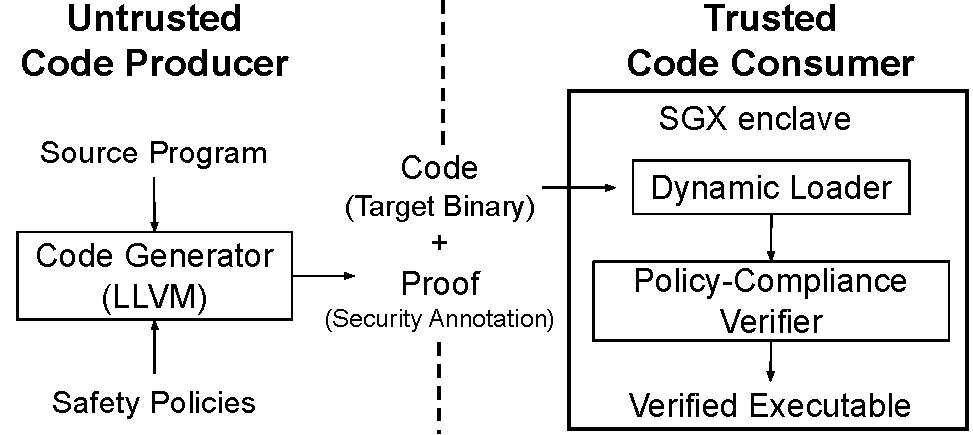
\includegraphics[scale=0.45]{figures/arch_overview.pdf}}
\centerline{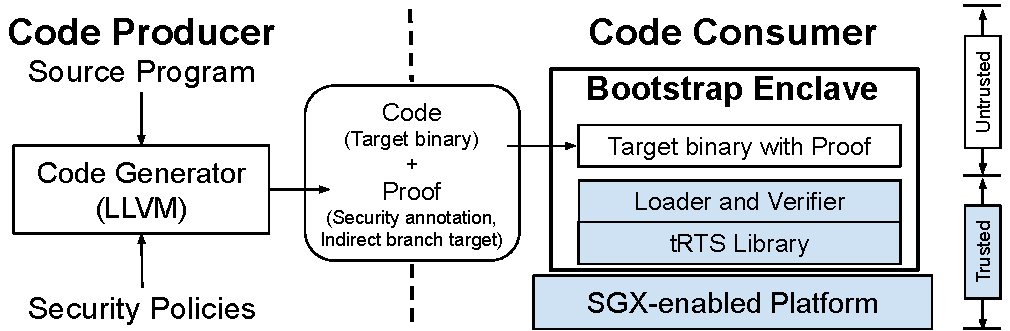
\includegraphics[scale=0.45]{figures/fg-bootstrap-layer.pdf}}
\caption{System overview}\label{fg-overview}
\vspace{-12pt}
\end{figure}

Instead, we construct a lightweight PCC-type scheme which includes an untrusted code producer and a trusted code consumer running in the bootstrap enclave (Fig.~\ref{fg-overview}). The overview design is derived from the original PCC idea while we have simplified it for our own purpose. The illustration of our design lists all components that are divided into two parts, trusted part and untrusted part. In our new PCC-based system, the proof is generated from the outside of the enclave during the compiling and can be verified at runtime inside. The inside verifier can cooperate with the outside compiler to make the verifier as lightweight as possible, using static verification of dynamic checks.
%\weijie{will unify them all into `verifier'}

In traditional PCC framework, the VCGen often exists as a compiler~\cite{colby2000certifying,leroy2006formal} or a sandbox~\cite{pirzadeh2010extended}, which is too heavy for limited executive resources. So here, we build our own lightweight PCC system to verify if a cloud service would leakage user’s data. Generally, we provide a code transformer for service code which needs to be verified, and a secure enclave for executing the verified service code. The only TCB in our design is the verifier code inside the enclave, including the dynamic-loader, the disassembler/rewriter (for rewritting structured guards), and the proof verifier (for checking verification hints). On the other hand, the whole trusted code consumer can be remotely attested (in Subsection~\ref{subsec-dynamicloader}), which can indirectly protect the integrity of for code provider, as well as the isolate valuable implementation detail from be accessed.

As mentioned above, to facilitate PCC framework working well in SGX and to make PCC more efficient, specifically to reduce the size of code consumer side, we move as much proof generation workload as possible to the code producer side, and leave as few verification workload as possible to the inside of the enclave.

\begin{figure*}[htbp]
\centerline{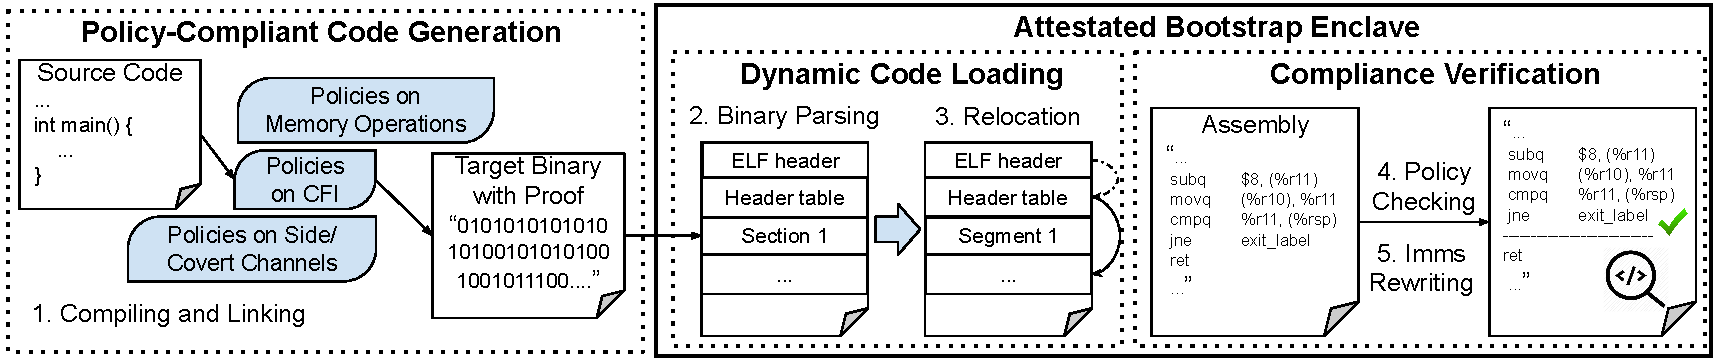
\includegraphics[scale=0.5]{figures/fg-workflow.pdf}}
\caption{Detailed framework and workflow}\label{fg-workflow}
%\wenhao{Typo: Attestated Bootstrap Enclave}
%\weijie{done. Thanks!}
\vspace{-15pt}
\end{figure*}
%\weijie{need some changes on the figure}

\vspace{3pt}\noindent\textbf{Workflow.} The workflow of our privacy-preserving TEE and PCC framework is shown as Figure~\ref{fg-workflow}. Unlike the typical interaction between the producer and consumer, the workflow encompasses several steps. 

First, the service code (target program) is instrumented using our own `code + proof' generator - a customized LLVM-based compiler (step 1,2). Then on the code consumer side, the loader source code and the verifier source code are compiled with SGX SDK to build the bootstrap enclave binary (step 3). Our loader can load and unload code after initialization (step 4), followed by being remote attested (step 5). Moreover, the `code + proof' can be transferred to code consumer where SGX is deployed, waiting for being dynamic loaded and rebased into the enclave (step 6). After being loaded, the verifier will rewrite some key immediate operands (Imm) and finally transfer the execution to the target program (step 7). 

\vspace{3pt}\noindent\textbf{Dynamic Code Loading and Unloading.} \label{subsec-dynamicloader}
%To ensure the bootstrap enclave's code can be completely public and can be attested, we propose a multi-step loader that can load and unload a generated `code + proof' dynamically. Unlike previous work, our proposed solution can resolve the problem that remote attestation conflicts with the dynamic relocation requirement~\cite{seo2017sgx}. Specifically, remote attestation requires code, data and security properties of the enclave to remain unchanged, while executing a private binary code needs relocation for execution, which is a modification to memory distribution. 
%Our proposal is based on the fact that binary code to be verified can not be trusted, so the measurement of the enclave should not include the untrusted code. Therefore, the code to be verified should be dynamically loaded and relocated after the bootstrap enclave is initiated. 
%\weijie{elaborates it later in Section Implementation}
%\vspace{3pt}\noindent\textbf{Separated Linking and Rebasing.} 
In our design, the linking procedures (linking and rebasing) of a target program are separated into both inside and outside the enclave respectively. SGX only accepts that code running inside an enclave is linked against the SGX SDK at build time. For a self-contained function (i.e., one does not use external elements), compiling and sending the bytes of the assembled code is enough. However, if the function uses external elements, a distributed mechanism is needed to map these elements into their corresponding positions at the enclave side. So we use separated linking and rebasing to assemble all the symbols of the entire code (including necessary libraries and dependencies) into one relocatable file (aka. linking), and then parse the symbols and load/relocate the code at runtime inside the enclave (aka. rebasing). Further, during the linkage procedure, we also load and relocate an indirect branch target entry list as part of the proof for later runtime verification.
%Note that legal jump addresses can not be settled until the rebasing procedure is completed because rebasing will modify the addresses of symbols.

The rebasing process starts with the bootstrap enclave receiving the generated binary code through a buffer. The dynamic loader's primary task is to rebase all of its symbols according to information in its relocation table. Therefore, the loader reads relocation tables in the code, updates symbol offsets in symbol tables, and loads symbols to addresses designated in relocation tables. After rebasing, the detailed memory layout is shown on the right side in Fig.~\ref{fg-dynloader}.




%\wenhao{can elaborate on this. The numbers are not in any order}

\subsection{Security Policies}\label{subsec-policies}
%\subsection{Security Policies for the Privacy Preserving Online Data Processing Scenario}\label{subsec-policies}

%Our general goal of defining safety policies is to design a Privacy-preserving TEE prototype on a service-oriented environment for data owner. Here, we make some rules to constrain our design.
In this scenario, the bootstrap enclave needs to enforce that the data will not be leaked by the untrusted service code, which is not exposed to the data provider. It can be achieved by enforcing several policies as follows. Notably, the policies put some constraints on the service code, yet we make a lot of effort on these constraints to ensure that the code functionality are intact and necessary for the CAT model.

\vspace{3pt}\noindent\textbf {Constraining Ecalls/Ocalls}. In such service-oriented scenarios, all the bridge functions should be public and attestable for normal use, we should make restrictions on them. The output is to be produced encrypted and the loader must deal with system calls via a trusted Ocall routine. All ECalls/OCalls will be audited and configured correctly by the bootstrap enclave.  

\vspace{2pt}\noindent$\bullet$\textit{ P0: Standard and Encrypted Output via legitimate Ocalls}. After the Remote Attestation and the session key exchange, messages sent from the enclave should be all encrypted. And for security consideration, they could be the same length to prevent further inference attacks.

\vspace{3pt}\noindent\textbf {Verifying Memory Operations}. In order to prevent data leakage during it being processed by a untrusted code provider, we need a verifier to check if this program is prone to write sensitive information from inside enclave to the outside world. 

\vspace{2pt}\noindent$\bullet$\textit{ P1: Preventing explicit memory stores to the outside of the enclave}. An enclave has the ability to write data outside of its EPC memory region arbitrarily. Therefore, the major policy is to prevent the untrusted code from copying the data across enclave boundaries. The policy-compliance verifier needs to ensure that the destinations of memory store instructions such as \texttt{MOV} are within the enclave address range (also known as the \texttt{ELRANGE}). %The first thing we should guarantee is no writes onto non-data section. In addition to check various memory write operations caused by instructions like MOV, we need to prevent another register save/spill operations that possibly push some register value to memory space.

\vspace{2pt}\noindent$\bullet$\textit{ P2: Preventing implicit memory stores to the outside of the enclave}. Illicit RSP register save/spill operations can do the trick of leaking sensitive information to memory via pushing a register value to an address specified by the stack pointer. 
    %To address this issue, stack operating instructions need be inspected so that the stack pointer never points to memory regions outside the enclave. 
    
\vspace{2pt}\noindent$\bullet$\textit{ P3: Preventing tampering of security-critical data within the bootstrap enclave}. This ensures that the code never reads or writes secrets in the SSA/TCS area, which is necessary because strong security properties no longer hold if the thread control structure data is used. In this case the verifier needs to ensure that the untrusted code does not tamper with this kind of data structure.
    %\item \textit{P4: does not read from or write to L’s memory}. %\weijie{User's private code does not load from L’s memory. } %\wenhao{auditing memory loads is heavy? We may need to argue the leakage is controlled?}

\vspace{3pt}\noindent\textbf{Constraining Control Transfers}. 
%In order to prevent attackers from bypassing our checks, we need do CFI checks on multiple aspects.\todo{on this part}
In our PCC-type scheme, the policy-compliance verifier performs static analysis of the untrusted code. It is essential to prevent attackers from dynamically redirecting the control flow at runtime, which may bypass the check performed when the code is initially loaded. In this respect, the following policies need to be enforced. 

\vspace{2pt}\noindent$\bullet$\textit{ P4: Data execution prevention for the RWX region}. In the currently SGX platforms that support only SGXv1 instructions, the untrusted code are loaded to pages with \texttt{RWX} properties. A software DEP scheme is needed to prevent the untrusted code from changing the code at runtime.

\vspace{2pt}\noindent$\bullet$\textit{ P5: Indirect branches shall not point to destinations that violate policies P1 to P4}. Such control flow integrity definitely should be guaranteed since the loaded code could be malicious so that it could bypass the mentioned policies. Therefore, this enforcement should be performed for all indirect control transfer instructions, including indirect calls, indirect jumps, and return instructions.
    %\item \textit{P6: Checking if control transfer targets are embedded in proof instrumentations}. If an attacker knows the details of the representation of proof (aka. those instrumentations inserted by our LLVM), he/she can exploit it and further sabotage the control flow.

\vspace{3pt}\noindent\textbf{Detecting leakage through AEX based side channels}. Side channels are difficult to eliminate and are severe threats to TEEs such as SGX. As shown in previous works, the abnormal AEXs can be used to detect many low-noise side channels within SGX, such as controlled channel attacks~\cite{xu2015controlled}, and same core L1/L2 cache attacks~\cite{chen2018racing}. We are not meant to design new side channel defenses, nevertheless we propose to transplant 
existing side channel detecting techniques, 
which illustrates the generality of the CAT model. 

%Side and covert channels often hide in the normal behaviors during program execution since the logic of service provider’s code would be very complicated. However, side channel prevention is not an easy task. Here we design some alternative policies for side channel mitigation.

\vspace{2pt}\noindent$\bullet$\textit{ Alternative P6: Detecting page faults with TSX support}. 

\vspace{2pt}\noindent$\bullet$\textit{ Alternative P7: Detecting AEX by monitoring the SSA}.

\vspace{3pt}\noindent\textbf{Multi-Usesr Isolation}. When protecting in-enclave time-sharing services, a big challenge is to prevent the service program infected by one user from victimizing another user, and the confidentiality of a user’s data left in the enclave to protect it from leaking to the subsequent user receiving the service.

\vspace{2pt}\noindent$\bullet$\textit{ P8: User data cleansing}. The purpose of the data cleansing and the exit sanitization is to reset the service state and clean up the old user’s data right after execution is done. Except the persistent data of the user, all other data will be cleaned up, together with the content of SSA and registers.

\subsection{Policy-Compliant Code Generation}
\label{subsec-producer}
In this section we present the design of the code generator, which given the source program can produce binary code that enforces the policies P1 to P5, and can be easily verified. The design of the policy verifier will be presented in Sec.~\ref{subsec:verify}. Since we do the verification at the assembly level and the target binary loaded in the bootstrap enclave will finally be disassembled, the code generator does not need to be trusted.

%When the target binary wants a syscall or the in-enclave service ends, the computing results need to be output in a standard format.
\vspace{3pt}\noindent\textbf{Enforcing P0}. The output message for the in-enclave service is encrypted using session key after RA. Before that, to construct the output message, the plaintext is padded to a constant length if have to. Meanwhile, the output functions are wrapped by our customized Ocall stubs. On the other hand, 37 common system calls are also wrapped with Ocall stubs for possible system interactions.\wenhao{we need to discuss: admitting arbitrary ocalls could lead to information leakage by ocall patterns}

%enforcing mem ops
\vspace{3pt}\noindent\textbf{Enforcing P1}. The generator instruments all storing instructions to check if they are writing to the memory out of the enclave. The code consumer inside the enclave confirms such security check instructions are in place.

\vspace{3pt}\noindent\textbf{Enforcing P2}. The generator prevents implicit memory write crossing the enclave boundaries by making sure the stack pointer never point to memory regions outside the enclave. It locates all the instructions modifying the stack pointer explicitly, and inserts instructions to check the validity of the stack pointer after them. The code consumer confirms the placement of these check instruction. Furthermore, the code consumer prevents implicit modification of the stack pointer by adding guard pages (i.e., pages granted no permissions) around the stack boundaries. 

\vspace{3pt}\noindent\textbf{Enforcing P3}. Similar to enforcing P1 and P2, the code generator further enforces that (both explicit and implicit) memory write operations cannot alter the security-critical data once the untrusted code is loaded and verified. These check instructions are verified by the code consumer inside the enclave. 

%enforcing CFI
\vspace{3pt}\noindent\textbf{Enforcing P4}. Similar to enforcing P1 and P2, the code generator and consumer enforce that (both explicit and implicit) memory write operations cannot modify the \texttt{RWX} pages.

\vspace{3pt}\noindent\textbf{Enforcing P5}. For indirect calls or indirect jumps, the code generator firstly extract all legal destination addresses of them. Theses addresses are stored in a specific data region. Then it instruments code to check the targets of all the indirect call/jump instructions in the code to ensure they only direct to addresses listed in the data region. These instruments can be efficiently verified by the in-enclave code consumer.

%enforcing side channel mitigations
\vspace{3pt}\noindent\textbf{Enforcing P6}.
We enforce P6 by introducing the idea of T-SGX~\cite{shih2017t}. As a compiler-level scheme that automatically transforms a normal enclave program into a secured one, T-SGX can isolate the fallback handler and other transaction control code, called springboard, from the original program’s code and data pages to ensure that exceptions including page faults and timer interrupts can only be triggered on the springboard. We take advantage of it and implement instruction wrappers that encompass all boundaries between any basic blocks and branches. The fallback route of the TSX wrapper records the number of transaction aborts, which ensures that if a threshold is exceeded, the program is forced to exit. 

\vspace{3pt}\noindent\textbf{Enforcing P7}.
We enforce P7 by retrofitting Hyperrace~\cite{chen2018racing}. However, unlike Hyperrace doing the physical-core co-location tests, here we only monitor how often the interrupts/AEXs happen. L1/L2 cache-based channel can be detected when certain number or more interrupts/AEXs occur in one basic block or every k instructions.

%enforcing multi-user isolation
\vspace{3pt}\noindent\textbf{Enforcing P8}. Before the bootstrap enclave is destroyed, all user data is cleared after the execution transferred back to the loader.

\subsection{Compliance Verification}
\label{subsec:verify}

Due to the thorough generated proof with compliance, the bootstrap enclave can quickly verify the validity of the proof, and it can compare the conclusions of the proof to its own security policy to determine whether the application is safe to execute.

\vspace{3pt}\noindent\textbf{Just-enough Disassembling.} Accurate and complete binary disassembly is a difficult problem in general due to indirect control flow transfers. We built a lightweight disassembler with the assistance of the compiler outside the enclave. Our disassembler starts with the program entry and follows the program control flow. When we encounter indirect control flow transfers such as indirect jumps and indirect calls, we use the valid target list provided by the compiler to find the targets of indirect control flows. Note that our verifier will ensure that there are runtime checks before every indirect control flow, which guarantees that the actual control flow targets are inside the list provided by the compiler. In this way, the untrusted compiler is not able to hide dangerous transfer targets by omitting them in the list. The runtime check ensures the integrity of the target list provided by the compiler.
}